\section{Dynamic Programming}

% https://www.sciencedirect.com/topics/computer-science/dynamic-programming

Dynamic programming is an optimization method based on the principle of optimality 
defined by Bellman in the 1950s: “An optimal policy has the property that whatever 
the initial state and initial decision are, the remaining decisions must constitute 
an optimal policy with regard to the state resulting from the first decision.”

It can be summarized simply as follows: {\bf \textcolor{magenta}{“every optimal policy consists only of 
optimal sub policies.”}}

This method is a variant of the “divide and conquer” method given that a solution 
to a problem depends on the previous solutions obtained from subproblems. The main 
and major difference between these two methods relates to the superimposition of 
subproblems in dynamic programming. A subproblem can be used to solve a number of 
different subproblems. In the “divide and conquer” approach, subproblems are 
entirely independent and can be solved separately. Moreover, recursion is used, 
unlike in dynamic programming where a combination of small subproblems is used to 
obtain increasingly larger subproblems.

To sum up, it can be said that the “divide and conquer” method works by following 
a top-down approach whereas dynamic programming follows a bottom-up approach.

How these two methods function can be illustrated and compared in two arborescent graphs.

\begin{figure}[!htb]
\centering
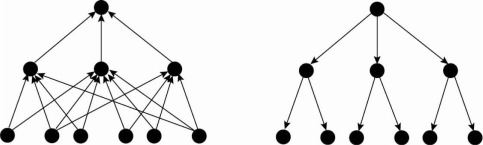
\includegraphics[scale=0.8]{pix/dnc_dp.jpg}
\caption{The methods: dynamic programming (left) and divide and conquer (right)}
%\label{fig:label}
\end{figure}




\subsection{Bellman backup equation}


\begin{tikzpicture}[->,>=stealth',level/.style={sibling distance = 5cm/#1,
  level distance = 1.5cm}] 
\node [arn_n] {33}
    child{ node [arn_r] (test0) {15}
        {
            child{ node [arn_n] {10}
                {
                % edge from parent node[above left] {$r$}
                edge from parent node[below left] (A) { \makebox[8em][l]{$q_\pi(s',a') \leftarrowtail a'$} }
                }
            }
            child{ node [arn_n] {20} }
            edge from parent node[below left] (A) { \makebox[4em][l]{$s'$} }
        } edge from parent node[left] {$r$} %for a named pointer
    }
    child{ node [arn_r] (test1) {47}
            child{ node [arn_n] {38} }
            child{ node [arn_n] {51} }
	}edge from parent node[left] (A) {\makebox[7em][l]{$q_\pi(s,a) \leftarrowtail s, a$}}
    
    ;

    %\filldraw[red] (A) circle[radius=1pt];
\end{tikzpicture}

Bellman Equations are recursive relationships among values that can be used 
to compute values.

\begin{equation}\label{bellman_equation_DP}
q_\pi(s,a) = r(s,a) + \gamma \sum_{s'\in \mathcal{S}}\mathcal{P}_{ss'}^a 
\sum_{a'\in \mathcal{A}} \pi(a'|s')q_n(s',a')
\end{equation}
记住这里$q_\pi(s,a)$是累加reward的期望,传统的rl的目标函数等价于使$q_\pi(s,a)$最大。
\begin{align}
\pi^* = \arg\max_\pi \mathbb{E}_{(s_t,a_t)\sim\rho_\pi}
\Big[ \sum_t \big(
\underbrace{r(s_t, a_t)}_{\text{reward}} + 
\underbrace{\alpha \mathcal{H}(\pi(\cdot | s_t))}_{\text{entropy}}
\big)\Big] \tag{\ref{maximum_entropy_objective}}
\end{align}

{\bf \textcolor{magenta}{这个公式还未澄清!}}

% file:///D:/mygit/ml/reinforcementLearning/refs/bellman/6%20Bellman%20Eqs%20and%20DP.pdf

\begin{figure}[!htb]
\centering
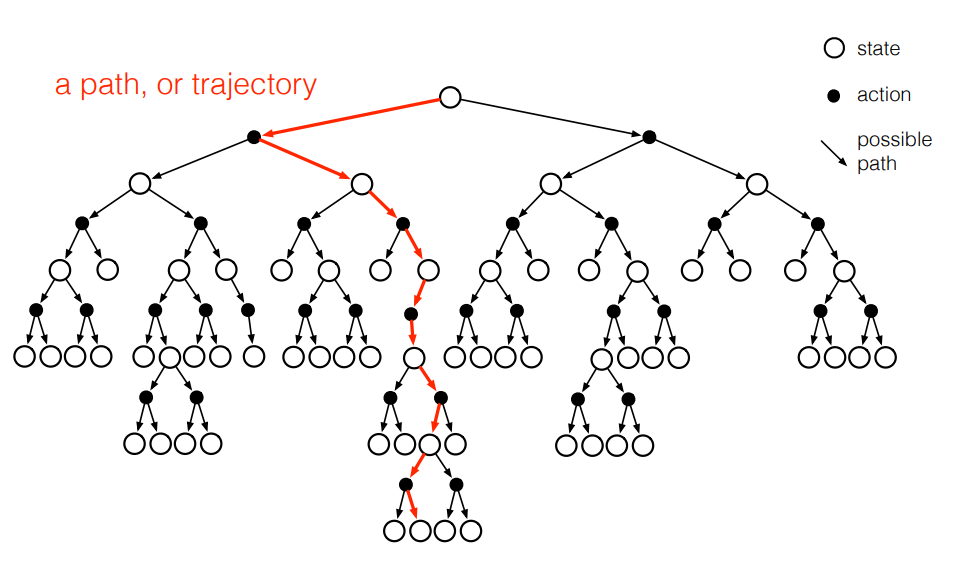
\includegraphics[scale=0.7]{pix/tee-transition-dynamics.png}
\caption{The tree of transition dynamics}
%\label{fig:label}
\end{figure}


\begin{figure}[!htb]
\centering
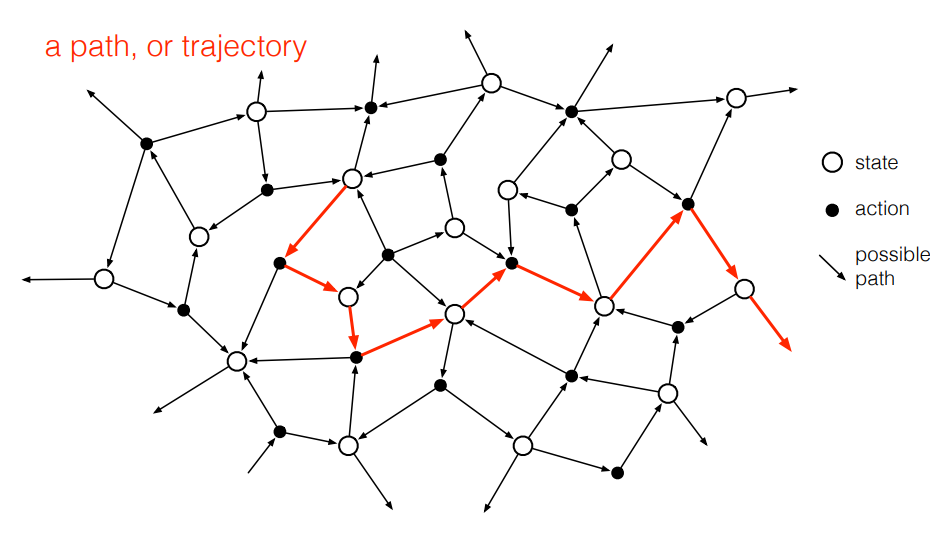
\includegraphics[scale=0.7]{pix/web-transition-dynamics.png}
\caption{The web of transition dynamics}
%\label{fig:label}
\end{figure}


\begin{figure}[!htb]
\centering
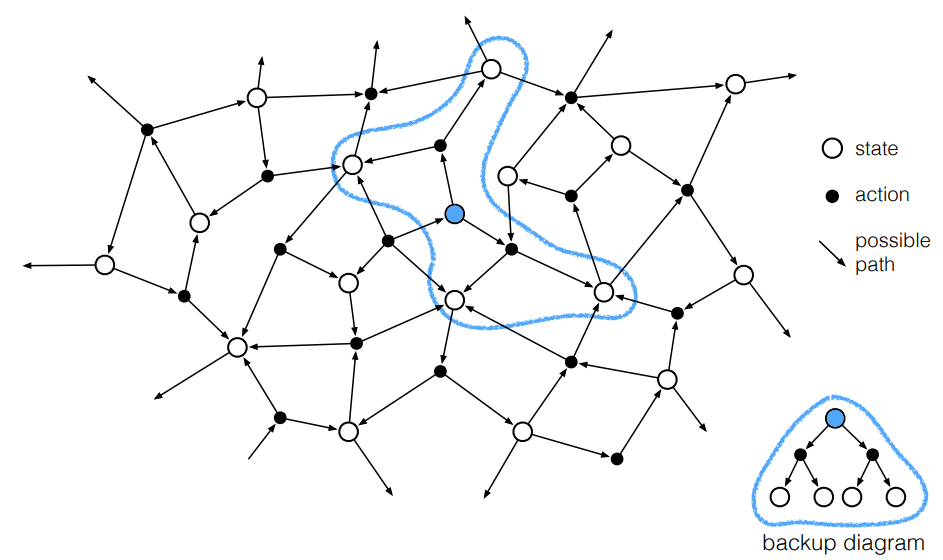
\includegraphics[scale=0.7]{pix/web2-transition-dynamics.png}
\caption{The web of transition dynamics}
%\label{fig:label}
\end{figure}


\subsection{4 Bellman-equation backup diagrams}

\begin{figure}[!htb]
\centering
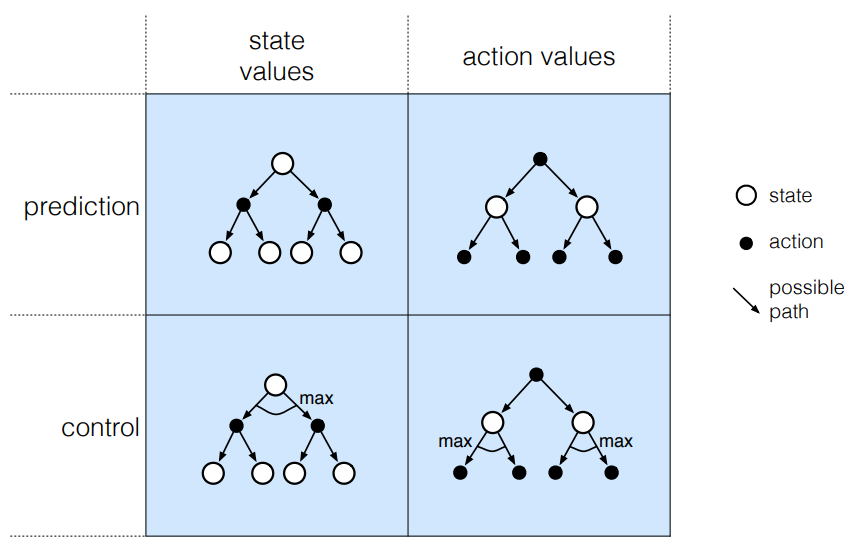
\includegraphics[scale=0.7]{pix/4-backup-diagrams.png}
\caption{4 Bellman-equation backup diagrams}
%\label{fig:label}
\end{figure}


\subsection{Bellman Equation for a Policy $\pi$}

这里的内容可对照 mdp 相应的部分。The return $G_t$ is the total discounted reward from $t$.
The discount rate $\gamma$ determines the present value of future rewards: a 
reward received $k$ time steps in the future is worth only $\gamma^{k-1}$ times 
what it would be worth if it were received immediately. And also, it provides 
mathematical convenience since as $k\rightarrow\infty$ then $\gamma^k\rightarrow 0$.

The basic idea:

\begin{align*}
G_t &= R_{t+1} + \gamma R_{t+2} + \gamma^2 R_{t+3} + \gamma^3 R_{t+4} + \cdots \\
&= R_{t+1} + \gamma \left( R_{t+2} + \gamma R_{t+3} + \gamma^2 R_{t+4} + \cdots \right) \\
&= R_{t+1} + \gamma G_{t+1}
\end{align}

So:
\begin{emp_box}
\begin{align*}
v_\pi(s) &= \mathbb{E}_\pi\left\{ G_t | S_t = s \right\} \\
&= \mathbb{E}_\pi\left\{ R_{t+1} + \gamma v_\pi\left( S_{t+1} \right) | S_t = s \right\}
\end{align}
\end{emp_box}

Or, without the expectation operator:
\begin{equation}\label{dp_set_policy_evaluation_backup}
v_\pi(s) = \sum_a \pi(a|s) \sum_{s',r} p(s', r | s, a) \left[ r + \gamma v_\pi(s') \right]
\end{equation}
This is a set of equations (in fact, linear), one for each state. The value function 
for $\pi$ is its unique solution.


\begin{figure}[!htb]
\centering
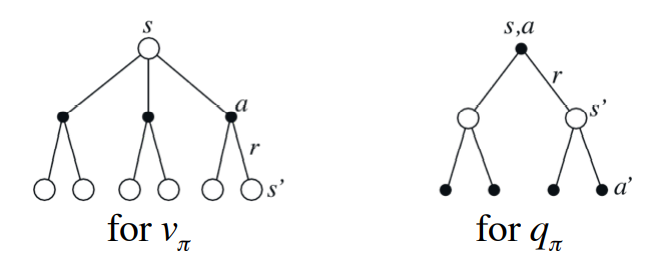
\includegraphics[scale=0.7]{pix/backup_diagrams.png}
\caption{Backup diagrams}
%\label{fig:label}
\end{figure}


\subsection{Bellman Optimality Equation for $q_*$}

\begin{align*}
q_*(s,a) &= \mathbb{E}\left[ R_{t+1} + \gamma\max_{a'}q_*\left( S_{t+1},a' \right) | S_t = s, A_t = a \right] \\
&= \sum_{s',r} p(s', r | s, a) \left[ r + \gamma\max_{a'}q_*(s',a') \right].
\end{align}

\begin{figure}[!htb]
\centering
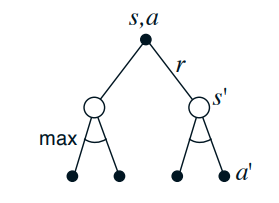
\includegraphics[scale=0.618]{pix/appendix/dp_relevant_backup_diagram.png}
\caption{The relevant backup diagram}
%\label{fig:label}
\end{figure}

\begin{emp_box}
$q_*$ is the unique solution of this system of nonlinear equations.
\end{emp_box}


\subsection{Iterative Methods}

$$
v_0\rightarrow v_1\rightarrow\cdots\rightarrow v_k\rightarrow v_{k+1}\rightarrow\cdots
\rightarrow v_\pi
$$

A sweep consists of applying a {\bf backup operation} to each state.

A {\bf full policy-evaluation backup}:

\begin{equation}\label{dp_full_policy_evaluation_backup}
v_{k+1}(s) = \sum_a \pi(a|s) \sum_{s',r} p(s', r | s, a) \left[ r + \gamma v_k(s') \right]
\qquad \forall s\in\mathcal{S}
\end{equation}

\begin{emp_box}
(\ref{dp_set_policy_evaluation_backup}) is a set of equations while 
(\ref{dp_full_policy_evaluation_backup}) is the state value backup for each state $s$.
\end{emp_box}

\subsubsection{What is meant by a "sweep" in Reinfocement Leraning?}
% https://stats.stackexchange.com/questions/499873/what-is-meant-by-a-sweep-in-reinfocement-leraning

What is meant by a sweep in value iteration or policy iteration in RL.

I saw it for the first time in Sutton's book. In the context they mentioned it is 
when computing value or policy iteration, but the inplace variant of the algorithms.

Sometimes, the value iteration, for example, is computed using two value tables. The 
one where you are computing the state values at time step $k$ and the previous one, 
at time step $k−1$. In contrast, the inplace algorithm does not use this auxiliary 
table; it updates the state values in the same table for both $k$ and $k−1$ time steps.

The sweeping comes from removing of the previous state value and writing in the same 
place the new one.

【{\bf 解读}】a sweep 似乎可以翻译为“置换迭代”, 似乎就是 sweep iteration。与之相关的研究参见文献
\cite{MCREYNOLDS1967565},其将动态规划问题写成积分方程的形式非常值得拜读。



\subsection{Policy Evaluation}
% http://www.incompleteideas.net/book/ebook/node41.html

First we consider how to compute the state-value function $V^\pi$ for an arbitrary 
policy $\pi$. This is called {\bf policy evaluation} in the DP literature. We also 
refer to it as the {\bf prediction problem}. Recall in RL that, for all $s \in \mathcal{S}$,

\begin{align}
V^\pi(s) &= \mathbb{E}_\pi\left\{ 
r_{t+1} + \gamma r_{t+2} + \gamma^2 r_{t+3} + \gamma^3 r_{t+4} + \cdots | s_t = s 
\right\} \notag \\
&= \mathbb{E}_\pi\left\{ r_{t+1} + \gamma V^\pi(s_{t+1}) | s_t = s \right\} \\ 
&= \sum_a \pi(s, a) \sum_{s'} \mathcal{P}_{ss'}^a \left[ \mathcal{R}_{ss'}^a + \gamma V^\pi(s') \right],
\label{policy_action_evaluation}
\end{align}
where $\pi(s, a)$ is the probability of taking action $a$ in state $s$ under policy 
$\pi$, and the expectations are subscripted by $\pi$ to indicate that they are 
conditional on $\pi$ being followed. The existence and uniqueness of $V^\pi$ are 
guaranteed as long as either $\gamma < 1$ or eventual termination is guaranteed from 
all states under the policy $\pi$.

If the environment's dynamics are completely known, then (\ref{policy_action_evaluation}) 
is a system of $|\mathcal{S}|$ simultaneous linear equations in $|\mathcal{S}|$ unknowns 
(the $V^\pi(s)$, $s\in\mathcal{S}$). In principle, its solution is a straightforward, if 
tedious(冗长的), computation. For our purposes, iterative solution methods are most suitable. 
Consider a sequence of approximate value functions $V_0, V_1, V_2, \ldots$, each mapping 
$\mathcal{S}$ to $\mathfrak{R}$. The initial approximation, $V_0$, is chosen arbitrarily 
(except that the terminal state, if any, must be given value $0$), and each successive 
approximation is obtained by using the Bellman equation for $V^\pi$ as an update rule:

\begin{align}
V_{k+1}(s) &= \mathbb{E}_\pi\left\{ r_{t+1} + \gamma V_k(s_{t+1}) | s_t = s \right\} \notag \\ 
&= \sum_a \pi(s, a) \sum_{s'} \mathcal{P}_{ss'}^a \left[ \mathcal{R}_{ss'}^a + \gamma V_k(s') \right],
\label{dp_bellman_equation}
\end{align}
for all $s\in\mathcal{S}$. Clearly, $V_k = V^\pi$ is a fixed point for this update 
rule because the Bellman equation for $V^*$ assures us of equality in this case. Indeed, 
the sequence ${V_k}$ can be shown in general to converge to $V^\pi$ as $k\rightarrow\infty$ 
under the same conditions that guarantee the existence of $V^\pi$. This algorithm is 
called {\bf iterative policy evaluation}.

To produce each successive approximation, $V_{k+1}$ from $V_k$, iterative policy 
evaluation applies the same operation to each state $s$: it replaces the old value of 
$s$ with a new value obtained from the old values of the successor states of $s$, and 
the expected immediate rewards, along all the one-step transitions possible under the 
policy being evaluated. We call this kind of operation a full backup. Each iteration 
of iterative policy evaluation backs up the value of every state once to produce the 
new approximate value function $V_{k+1}$. There are several different kinds of full 
backups, depending on whether a state (as here) or a state-action pair is being backed 
up, and depending on the precise way the estimated values of the successor states are 
combined. All the backups done in DP algorithms are called full backups because they 
are based on all possible next states rather than on a sample next state. The nature 
of a backup can be expressed in an equation, as above, or in a backup diagram like 
those introduced in Chapter \ref{rl_basics}. For example, Figure 
\ref{fig:backup_diagrams_rl}a is the backup diagram corresponding to the full backup 
used in iterative policy evaluation.

To write a sequential computer program to implement iterative policy evaluation, as 
given by (\ref{dp_bellman_equation}), you would have to use two arrays, one for the 
old values, $V_k(s)$, and one for the new values, $V_{k+1}(s)$. This way, the new 
values can be computed one by one from the old values without the old values being 
changed. Of course it is easier to use one array and update the values "in place," 
that is, with each new backed-up value immediately overwriting the old one. Then, 
depending on the order in which the states are backed up, sometimes new values are 
used instead of old ones on the right-hand side of (\ref{dp_bellman_equation}). This 
slightly different algorithm also converges to $V^\pi$; in fact, it usually converges 
faster than the two-array version, as you might expect, since it uses new data as 
soon as they are available. We think of the backups as being done in a sweep through 
the state space. For the in-place algorithm, the order in which states are backed up 
during the sweep has a significant influence on the rate of convergence. We usually 
have the in-place version in mind when we think of DP algorithms.

Another implementation point concerns the termination of the algorithm. Formally, 
iterative policy evaluation converges only in the limit, but in practice it must be 
halted short of this. A typical stopping condition for iterative policy evaluation 
is to test the quantity $\max_{s\in\mathcal{S}}|V_{k+1}(s)-V_k(s)|}$ after each sweep 
and stop when it is sufficiently small. Figure \ref{fig:dp_iterative_policy_evaluation} 
gives a complete algorithm for iterative policy evaluation with this stopping criterion.

\begin{figure}[!htb]
\centering
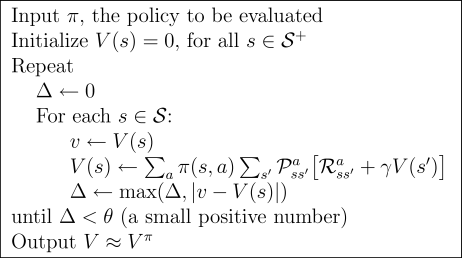
\includegraphics[scale=0.618]{pix/appendix/dp_iterative_policy_evaluation.png}
\caption{Iterative policy evalution}
\label{fig:dp_iterative_policy_evaluation}
\end{figure}

\subsection{Example: Gridworld}

Consider the $4\times 4$ gridworld shown in figure \ref{fig:dp_gridworld}.

\begin{figure}[!htb]
\centering
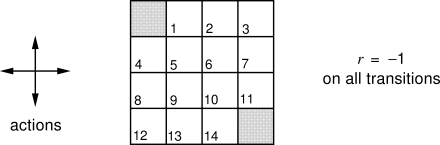
\includegraphics[scale=0.618]{pix/appendix/dp_gridworld.png}
\caption{Gridworld}
\label{fig:dp_gridworld}
\end{figure}

The nonterminal states are $\mathcal{S}={1,2,\ldots,14}$. There are four actions 
possible in each state, $\mathcal{A}={\text{up},\text{down},\text{right},\text{left}}$, 
which deterministically cause the corresponding state transitions, except that actions 
that would take the agent off the grid in fact leave the state unchanged. Thus, for 
instance, $\mathcal{P}_{5,6}^{\text{right}}=1$, $\mathcal{P}_{5,10}^{\text{right}}=0$, 
and $\mathcal{P}_{7,7}^{\text{right}}=1$. This is an undiscounted, episodic task. The 
reward is $-1$ on all transitions until the terminal state is reached. The terminal 
state is shaded in the figure (although it is shown in two places, it is formally one 
state). The expected reward function is thus $\mathcal{R}_{ss'}^a=-1$ for all states 
$s,s'$ and actions $a$. Suppose the agent follows the equiprobable random policy (all 
actions equally likely). The left side of Figure \ref{fig:dp_gridworld_convergence} 
shows the sequence of value functions ${V_k}$ computed by iterative policy evaluation. 
The final estimate is in fact $V^\pi$, which in this case gives for each state the 
negation of the expected number of steps from that state until termination.

\begin{figure}[!htb]
\centering
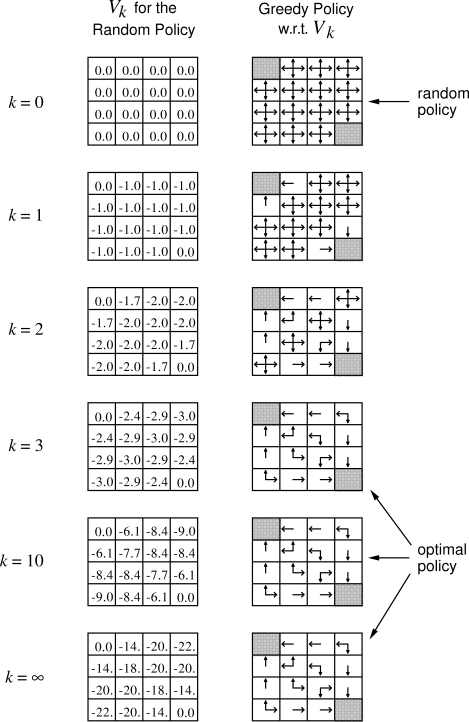
\includegraphics[scale=0.6]{pix/appendix/dp_gridworld_convergence.png}
\caption{Convergence of iterative policy evaluation on a small gridworld. The left column is the sequence of approximations of the state-value function for the random policy (all actions equal). The right column is the sequence of greedy policies corresponding to the value function estimates (arrows are shown for all actions achieving the maximum). The last policy is guaranteed only to be an improvement over the random policy, but in this case it, and all policies after the third iteration, are optimal.}
\label{fig:dp_gridworld_convergence}
\end{figure}


\subsection{Example: Gambler's Problem}
% https://github.com/kraftpunk97/gamblers-problem

A dynamic programming solution to the classic gambler's problem introduced in 
Sutton and Barton's RL book.

Problem statement - The gambler has a stake s between 0 and 100. At each play 
he wagers an integer <= $s$. He wins that much with prob $p$, else he loses that 
much. If he builds his stake to $100$ he wins (thus he never wagers more than 
($- 100$ s)); if his stake falls to $0$ he loses.

The solution (Or rather one of the possible solutions. It all boils down to the 
finer details, like how ties are broken the compiler etc...)

\begin{figure}[!htb]
\centering
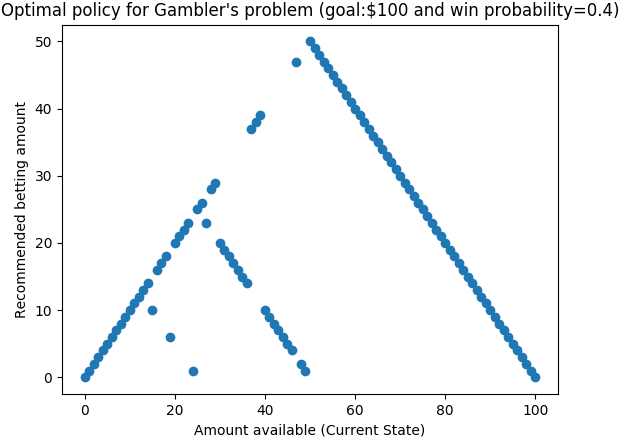
\includegraphics[scale=0.6]{pix/appendix/dp_gambler_s_problem_solution.png}
\caption{solution to the Gambler's Problem.}
\label{fig:dp_gambler_s_problem_solution}
\end{figure}

\begin{itemize}
%\setlength{\itemsep}{0pt}
%\setlength{\parsep}{0pt}
\setlength{\parskip}{0pt}
\item[-]
Gambler can repeatedly bet \$ on a coin flip

\item[-]
Heads he wins his stake, tails he loses it

\item[-]
Initial capital $\in \{\$1, \$2, \ldots, \$99\}$

\item[-]
Gambler wins if his capital becomes \$100 \\
loses if it becomes \$0

\item[-]
Coin is unfair \\
$\rightarrow$ Heads (gambler wins) with probability $p = .4$

\item[-]
States, Actions, Rewards?

\end{itemize}

\begin{figure}[!htb]
\centering
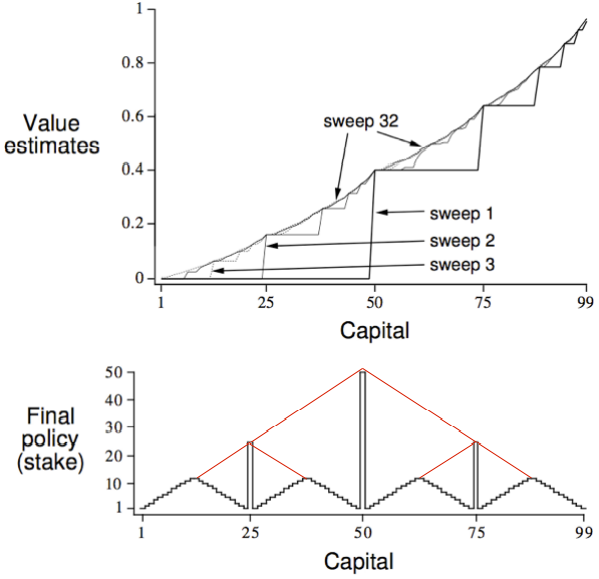
\includegraphics[scale=0.6]{pix/appendix/dp_gambler_s_problem_solution_1.png}
\caption{solution to the Gambler's Problem.}
%\label{fig:dp_gambler_s_problem_solution}
\end{figure}


\subsection{Example: Log Gambler - Model}
% https://utw11041.utweb.utexas.edu/ORMM/computation/unit/dynamic_programming/examples/gambler/model.html

This example comes from a book {\bf Introduction to Stochastic Programming} by 
Sheldon M. Ross, (Academic Press, 1982). In the book the problem is described with 
a continuous nonnegative state unbounded from above. The action variable is also 
continuous. For our purposes we will discretize both state and action.

\begin{emp_box}
A gambler is playing a game that has two results, win or lose. He can bet any amount 
up to his entire wealth. If he wins the amount of the bet is added to his wealth, and 
if he loses the amount of the bet is subtracted from his wealth. The gambler's goal 
is to maximize the log of his wealth after a fixed number of plays.
\end{emp_box}

To make analysis possible, we define the gambler's wealth as the state variable 
measured in whole dollars. We restrict the gambler's wealth to be less than the 
quantity $M$. Bets are measured in dollars and in this model the amount of the bet is 
the action variable. Bets are restricted so that the gambler can never bet an amount 
that would reduce his wealth to less than $\$1$ or more than $M$. There are $N$ plays 
in the game and the objective is to maximize the log of the wealth after play $N$.
\begin{emp_box}
\begin{itemize}
%\setlength{\itemsep}{0pt}
%\setlength{\parsep}{0pt}
\setlength{\parskip}{0pt}
\item[-]
Wealth at the beginning of the game: $S_0$

\item[-]
Wealth after $n$ plays: $S_n$

\item[-]
Bet at play $n$: $x_n$

\item[-]
Wealth after play $n$: $S_n = S_{n-1} \pm x_n$

\item[-]
Maximum wealth: $M$

\item[-]
Number of plays: $N$

\item[-]
Objective: $\max\left[\ln(S_N)\right]

\end{itemize}
\end{emp_box}


\subsubsection{States}

The states are defined with a single state variable. The state definition region on 
the model worksheet is shown below. Cell F14 holds the value of the current state, 
$10$. For the example we choose to limit the wealth to $\$20$. The lower bound on 
the state is in F18, and the upper bound is in F19.

\begin{figure}[!htb]
\centering
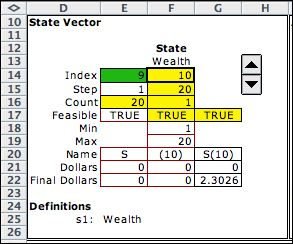
\includegraphics[scale=0.6]{pix/appendix/dp_gambler_state.jpg}
\caption{Gambler's state.}
\label{fig:dp_gambler_state}
\end{figure}

The example illustrates a new feature of the DP Models add-in, the ability to define 
the values for the final state. This is important for finite time horizon problems. 
For the Gambler problem, the only objective concerns the value at the final state. 
The goal is to maximize the log of the wealth at the end of the time horizon, 20 
plays for the example shown above.

After enumeration the state list appears as below. The Final Dollars column is 
computed as ln(final wealth).

\begin{figure}[!htb]
\centering
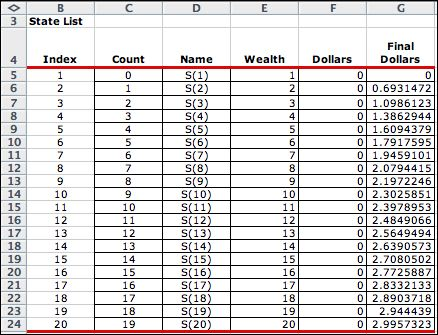
\includegraphics[scale=0.6]{pix/appendix/dp_gambler_statelist.jpg}
\caption{Gambler's state list.}
\label{fig:dp_gambler_statelist}
\end{figure}

\subsubsection{Actions}

The action is the amount the gambler bets on a given play. The range of bets is defined 
in the action element. The goal of the DP is to select bets at each state to maximize 
the log of the wealth at the end of the game.

\begin{figure}[!htbp]
\centering
\begin{minipage}{0.49\linewidth}
  \centering
  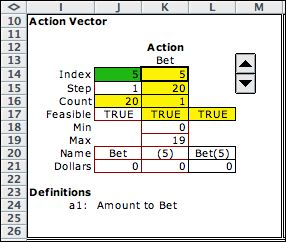
\includegraphics[width=0.618\linewidth]{pix/appendix/dp_gambler_action.jpg}
  \caption{Gambler action.}
  \label{fig:dp_gambler_action}
\end{minipage}%
\begin{minipage}{0.49\linewidth}
  \centering
  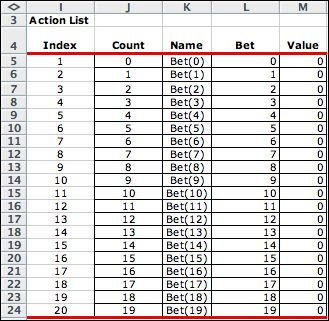
\includegraphics[width=0.618\linewidth]{pix/appendix/dp_gambler_action_list.jpg}
  \caption{Gambler action list.}
  \label{fig:dp_gambler_action_list}
\end{minipage}
\end{figure}

\subsubsection{Events}

The event indicates whether the bet wins or loses. The probability of winning is a 
parameter of the system, stored in Q24. The example assumes the probability of winning 
is $0.6$ with a corresponding probability of losing of $0.4$. The summary starting 
in column $S$ shows that the combination of elements, S(10)/Bet(5)/Win, is feasible.

\begin{figure}[!htbp]
\centering
\begin{minipage}{0.49\linewidth}
  \centering
  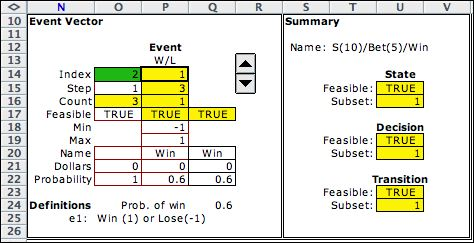
\includegraphics[width=0.618\linewidth]{pix/appendix/dp_gambler_event.jpg}
  \caption{Gambler event.}
  \label{fig:dp_gambler_event}
\end{minipage}%
\begin{minipage}{0.49\linewidth}
  \centering
  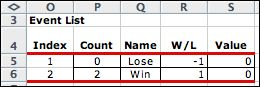
\includegraphics[width=0.618\linewidth]{pix/appendix/dp_gambler_event_list.jpg}
  \caption{Gambler event list.}
  \label{fig:dp_gambler_event_list}
\end{minipage}
\end{figure}


\subsubsection{Decisions}



\subsection{Example: Log Gambler - Solution}
% https://utw11041.utweb.utexas.edu/ORMM/computation/unit/dynamic_programming/examples/gambler/solve.html



\subsection{How to solve a Dynamic Programming Problem ?}
% https://www.geeksforgeeks.org/solve-dynamic-programming-problem/


\subsection{The successive sweep method and dynamic programming}
\cite{MCREYNOLDS1967565}
% 该文已下载,位于 ml/reinforcementLearning/refs/successive_sweep.pdf


\subsubsection{The problem}

The optimal control problem that shall be considered in this subsection will 
be the Bolza problem. It consists of finding certain unknown control functions 
$u(t) = (u_1(t),\ldots,u_m(t))$ and control parameters $a = (a_1,\ldots, a_p)$ 
that optimize the performance of some physical system. The performance of the 
system is measured by a performance index $J$ which assumes the general form
\begin{equation}\label{DP_performance_index_general_form}
J=\phi(x(t_N), a, t_N) + \int_{t_0}^{t_N} L(x(t),u(t),a,t) dt.
\end{equation}
The vector $x(t) = \left(x_1(t), x_2(t),\ldots, x_n(t)\right)$ denotes the state 
of the physical system. The control functions and the control parameters affect 
the state of the system through a set of system equations
\begin{equation}
\dot{x} = f(x,u,a,t). \label{DP_system_equations}
\end{equation}

For the purposes of this subsection the time interval $(t_0, t_N)$ will be assumed 
fixed. The initial state will be assumed given by the equations
\begin{equation}
x(t_0) = x_0 \text{specified}.
\end{equation}

An optimal control problem is usually complicated by the presence of side 
contraints. Of the various possible types of constraints, we shall consider the 
following kinds: 
\begin{align}
\Psi_0 = \Psi(x({t_N}), a, t_N) + \int_{t_0}^{t_N} M(x(t), u(t), a, t) dt \\
C(x, u, a, t) \leq 0. \label{DP_side_contraints_inequality}
\end{align}

A set of functions and parameters $(x(t), u(t), a)$ that satisfies Eqs. 
(\ref{DP_system_equations})-(\ref{DP_side_contraints_inequality}) 
over $[t_0, t_N]$ is referred to as an “admissible solution.” The problem in 
optimal control is to find the admissible solution for which the performance 
index attains its maximum (or minimum). 


